%\documentclass[a4paper,10pt]{article}

%\usepackage[a4paper, margin=1in]{geometry} % Set 1 inch margins (adjust as needed)
%\usepackage{tikz,tikz-3dplot}
%\usepackage{subcaption}
%\usepackage{hyperref}
%\usepackage{algorithm2e}
%\usepackage{graphicx}
%\usepackage{listings}
%\usetikzlibrary{trees}

%% \lstdefinestyle{BashInputStyle}{
%%   language=bash,
%%   basicstyle=\small\ttfamily,
%% %  numbers=left,
%% %  numberstyle=\tiny,
%% %  numbersep=3pt,
%%   frame=single,
%%   columns=fullflexible,
%%   backgroundcolor=\color{yellow!10},
%%   linewidth=0.95\linewidth,
%%   xleftmargin=0.05\linewidth,
%%   keepspaces=true,
%%   breaklines=true,
%%   framesep=5pt,
%%   rulecolor=\color{black!30},
%%   aboveskip=10pt,
%% }

%\begin{document}

\section{Introduction}
NekMesh is described in its paper \cite{NekMesh_paper} as "an
open-source mesh generation package which is designed to enable the
generation of valid, high-quality curvilinear meshes of complex,
three-dimensional geometries for performing high-order simulations."
To summarise, NekMesh is comprised of various Input, Process and
Output modules, and the workflow is to run 1) one input module 2) $n$
process modules 3) one output module. Before learning about the three
module types, we need a good understanding of the theory underpinning
the NekMesh format.

\section{Theory}
\subsection{Mesh Hierarchy}
The most fundamental thing we need to understand is how meshes are stored. The hierarchy of components that form a mesh is given in fig. \ref{fig:NekMesh_hierarchy}\\

\begin{figure}[h!]
  \centering
  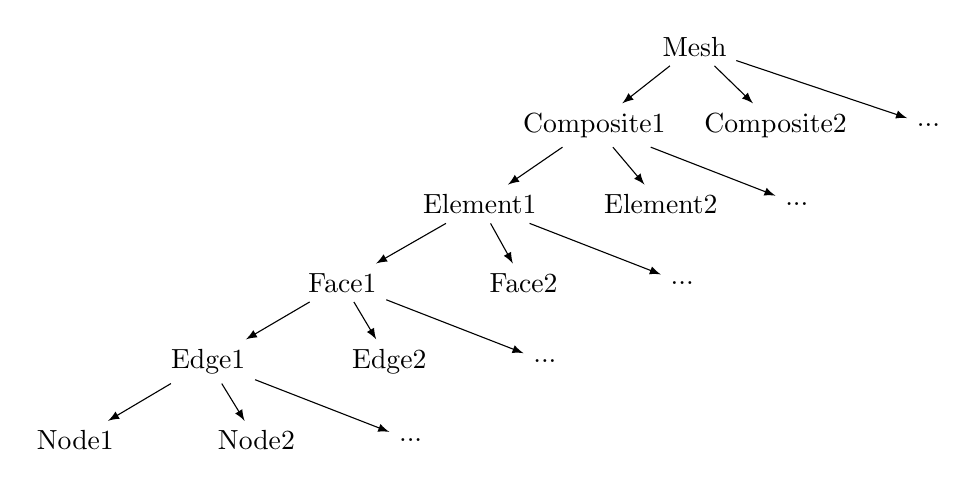
\begin{tikzpicture}[
  sibling distance=23mm, 
  level distance=10mm,
  edge from parent/.style={draw,-latex}, 
  grow=south,
  every node/.style={anchor=west}
]

% Root node
\node {Mesh}
  child {node {Composite1}
    child {node {Element1}
      child {node {Face1}
        child {node {Edge1}
          child {node {Node1}}
          child {node {Node2}}
          child {node {...}}}
        child {node {Edge2}}
        child {node {...}}}
      child {node {Face2}}
      child {node {...}}}
    child {node {Element2}}
    child {node {...}}}
  child {node {Composite2}}
  child [sibling distance=27mm]{node {...}};

\end{tikzpicture}
  \caption{}
  \label{fig:NekMesh_hierarchy}
\end{figure}

Meshes have a \textbf{dimensionality} of their own (eg. for a surface
mesh \texttt{expDim = 2}, for a volume mesh \texttt{expDim = 3}), and
exist in n-dimensional physical space (\texttt{physDim}, where
{\texttt{physDim} $\geq$ \texttt{expDim}). \textbf{Composites} are
  collections of elements. For elements which have the same
  dimensionality as the physical space they are in, they are grouped
  by their type. \textbf{Note:} boundary tri and quad elements are all
  grouped into a singular composite. \textbf{Boundary element} are
  elements that form the boundary of a mesh area/volume. These are one
  dimension lower than the physical dimension (eg. in 3D space, mesh
  volumes have boundary \textit{surfaces}).

\subsection{Vertex node ordering rules}
\label{sect:node_ordering}
\subsubsection{Collapsed points} 
NekMesh supports quadrilateral (quad) and triangular (tri) 2D
elements, and tetrahedral (tet), prism, pyramid (pyra) and hexahedral
(hex) 3D element. Elements with tri faces (all except quads and hexes)
use a collapsed coordinate systems (fig. \ref{fig:collapsed_coords})
\cite{textbook}, a feature which introduces constraints when
assembling and connecting 3D elements.

In the code, we indicate which node in a tri face is the collapsed point by giving it the highest node id (in \texttt{InputCGNS.cpp} and \texttt{InputStar.cpp} the node ordering is done in the function \texttt{ResetNodes}). Note that the relative ordering between nodes in \textit{different faces} (even if in the same element) has no affect.

\begin{figure}[h!]
    \centering
    \begin{subfigure}[b]{0.45\textwidth}
        \centering
        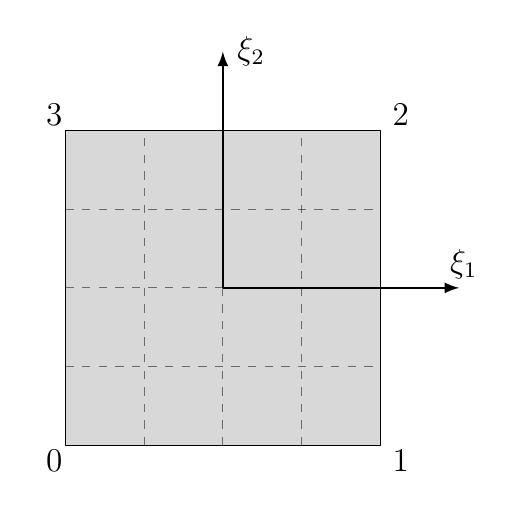
\begin{tikzpicture}[line join=bevel,scale=2,>=latex]
  \coordinate (n0) at (-1,-1);
  \coordinate (n1) at (1,-1);
  \coordinate (n2) at (1,1);
  \coordinate (n3) at (-1,1);

  \coordinate (n4) at (-0.5, -1);
  \coordinate (n5) at (0, -1);
  \coordinate (n6) at (0.5, -1);

  \coordinate (n7) at (1, -0.5);
  \coordinate (n8) at (1, 0);
  \coordinate (n9) at (1, 0.5);

  \coordinate (n10) at (0.5, 1);
  \coordinate (n11) at (0, 1);
  \coordinate (n12) at (-0.5, 1);

  \coordinate (n13) at (-1, 0.5);
  \coordinate (n14) at (-1, 0);
  \coordinate (n15) at (-1, -0.5);

  \coordinate (C) at (0, 0);
  \coordinate (j) at (0, 1.5);
  \coordinate (i) at (1.5, 0);

  \begin{scope}[blend mode=multiply]
    \fill[black!30,fill opacity=0.5] (n0) -- (n1) -- (n2) -- (n3) -- cycle;
  \end{scope}
  
  \draw (n0) -- (n1) -- (n2) -- (n3) -- cycle;
  \draw[dashed,opacity=0.5] (n4) -- (n12);
  \draw[dashed,opacity=0.5] (n5) -- (n11);
  \draw[dashed,opacity=0.5] (n6) -- (n10);
  \draw[dashed,opacity=0.5] (n15) -- (n7);
  \draw[dashed,opacity=0.5] (n14) -- (n8);
  \draw[dashed,opacity=0.5] (n13) -- (n9);

  \draw[thick, ->] (C) -- (i);
  \draw[thick, ->] (C) -- (j);
  \node at (1.5, 0.15) {\fontsize{12}{12} \selectfont $\xi_1$};
  \node at (0.15, 1.5) {\fontsize{12}{12} \selectfont $\xi_2$};
  \node at (-1.1, -1.1) {\fontsize{12}{12} \selectfont $0$};
  \node at (1.1, -1.1) {\fontsize{12}{12} \selectfont $1$};
  \node at (1.1, 1.1) {\fontsize{12}{12} \selectfont $2$};
  \node at (-1.1, 1.1) {\fontsize{12}{12} \selectfont $3$};

  
\end{tikzpicture}

        \caption{Coordinate system for the reference quadrilateral.}
        \label{fig:quad_coords}
    \end{subfigure}
    \hfill
    \begin{subfigure}[b]{0.45\textwidth}
        \centering
        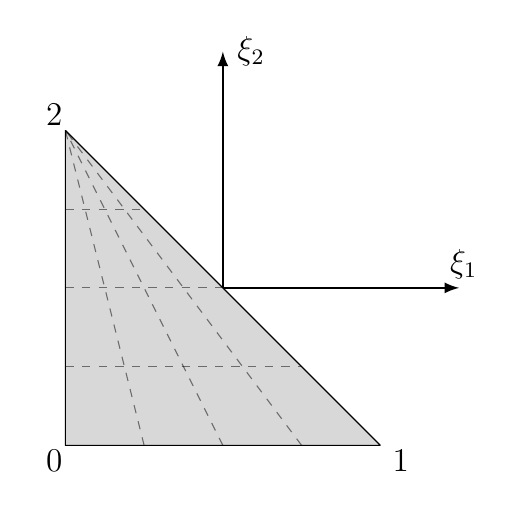
\begin{tikzpicture}[line join=bevel,scale=2,>=latex]
  \coordinate (n0) at (-1,-1);
  \coordinate (n1) at (1,-1);
  \coordinate (n2) at (-1,1);

  \coordinate (n3) at (-0.5, -1);
  \coordinate (n4) at (0, -1);
  \coordinate (n5) at (0.5, -1);

  \coordinate (n6) at (0.5, -0.5);
  \coordinate (n7) at (0, 0);
  \coordinate (n8) at (-0.5, 0.5);

  \coordinate (n9) at (-1, 0.5);
  \coordinate (n10) at (-1, 0);
  \coordinate (n11) at (-1, -0.5);

  \coordinate (C) at (0, 0);
  \coordinate (j) at (0, 1.5);
  \coordinate (i) at (1.5, 0);

  \begin{scope}[blend mode=multiply]
    \fill[black!30,fill opacity=0.5] (n0) -- (n1) -- (n2) -- cycle;
  \end{scope}
  
  \draw (n0) -- (n1) -- (n2) -- cycle;
  \draw[dashed,opacity=0.5] (n3) -- (n2);
  \draw[dashed,opacity=0.5] (n4) -- (n2);
  \draw[dashed,opacity=0.5] (n5) -- (n2);
  \draw[dashed,opacity=0.5] (n11) -- (n6);
  \draw[dashed,opacity=0.5] (n10) -- (n7);
  \draw[dashed,opacity=0.5] (n9) -- (n8);

  \draw[thick, ->] (C) -- (i);
  \draw[thick, ->] (C) -- (j);
  \node at (1.5, 0.15) {\fontsize{12}{12} \selectfont $\xi_1$};
  \node at (0.15, 1.5) {\fontsize{12}{12} \selectfont $\xi_2$};
  \node at (-1.1, -1.1) {\fontsize{12}{12} \selectfont $0$};
  \node at (1.1, -1.1) {\fontsize{12}{12} \selectfont $1$};
  \node at (-1.1, 1.1) {\fontsize{12}{12} \selectfont $2$};
  
\end{tikzpicture}

        \caption{Collapsed coordinate system for the reference triangle. Node 2 is considered the 'collapsed point'.}
        \label{fig:collapsed_coords}
    \end{subfigure}
    \caption{Coordinate systems for 2D elements/faces.}
    \label{fig:coords}
\end{figure}

\subsubsection{Tri interface rule}
This rule simply states that when tri faces on two elements meet, the collapsed point must be the same for each tri (fig. \ref{fig:tri_interface_rule}).

\begin{figure}[h!]
    \centering
    \begin{subfigure}[b]{0.45\textwidth}
        \centering
        \tdplotsetmaincoords{70}{60}

\begin{tikzpicture}[line join=bevel,tdplot_main_coords,scale=1.25,>=latex]

  \coordinate (a) at (-1, 1.5,-1);
  \coordinate (b) at ( 1, 1.5,-1);
  \coordinate (c) at ( 1, 3.5,-1);
  \coordinate (d) at (-1, 3.5,-1);
  \coordinate (e) at (-1, 1.5, 1);
  \coordinate (f) at (-1, 3.5, 1);
  
  \coordinate (ab1) at (-0.33, 1.5, -1);
  \coordinate (ab2) at (0.33, 1.5, -1);
  \coordinate (ae1) at (-1, 1.5, -0.33);
  \coordinate (ae2) at (-1, 1.5, 0.33);
  \coordinate (be1) at ( 0.33, 1.5, -0.33);
  \coordinate (be2) at (-0.33, 1.5, 0.33);
  
  \coordinate (dc1) at (-0.33, 3.5, -1);
  \coordinate (dc2) at (0.33, 3.5, -1);
  \coordinate (df1) at (-1, 3.5, -0.33);
  \coordinate (df2) at (-1, 3.5, 0.33);
  \coordinate (cf1) at (0.33, 3.5, -0.33);
  \coordinate (cf2) at (-0.33, 3.5, 0.33);
  
  \begin{scope}[blend mode=multiply]
    \fill[green!30,fill opacity=0.3] (a) -- (b) -- (e) -- cycle;
    \fill[black!30,fill opacity=0.3] (d) -- (c) -- (f) -- cycle;
  \end{scope}
  
  \draw(e) -- (b) -- (a) -- cycle;
  \draw (b) -- (c) -- (f) -- (e);
  \draw[dashed,opacity=0.5] (c) -- (d) -- (a);
  \draw[dashed,opacity=0.5] (d) -- (f);
  
  \draw [green!100](ab1) -- (e);
  \draw [green!100](ab2) -- (e);
  \draw [green!100](ae1) -- (be1);
  \draw [green!100](ae2) -- (be2);
  \draw [black!50](dc1) -- (f);
  \draw [black!50](dc2) -- (f);
  \draw [black!50](df1) -- (cf1);
  \draw [black!50](df2) -- (cf2);


  \coordinate (A) at (-1,-1,-1);
  \coordinate (B) at ( 1,-1,-1);
  \coordinate (C) at ( 1, 1,-1);
  \coordinate (D) at (-1, 1,-1);
  \coordinate (E) at (-1,-1, 1);
  \coordinate (F) at (-1, 1, 1);

  \coordinate (AB1) at (-0.33, -1, -1);
  \coordinate (AB2) at (0.33, -1, -1);
  \coordinate (AE1) at (-1,-1,-0.33);
  \coordinate (AE2) at (-1,-1,0.33);
  \coordinate (BE1) at ( 0.33,-1,-0.33);
  \coordinate (BE2) at ( -0.33,-1,0.33);

  \coordinate (DC1) at (-0.33, 1, -1);
  \coordinate (DC2) at (0.33, 1, -1);
  \coordinate (DF1) at (-1,1,-0.33);
  \coordinate (DF2) at (-1,1,0.33);
  \coordinate (CF1) at ( 0.33,1,-0.33);
  \coordinate (CF2) at ( -0.33,1,0.33);
  
  \begin{scope}[blend mode=multiply]
    \fill[black!30,fill opacity=0.3] (A) -- (B) -- (E) -- cycle;
    \fill[green!30,fill opacity=0.3] (D) -- (C) -- (F) -- cycle;
  \end{scope}
  
  \draw (A) -- (B) -- (E) -- cycle;
  \draw (B) -- (C) -- (F) -- (E);
  \draw[dashed,opacity=0.5] (C) -- (D) -- (A);
  \draw[dashed,opacity=0.5] (D) -- (F);

   \draw [black!50](AB1) -- (E);
   \draw [black!50](AB2) -- (E);
   \draw [black!50](AE1) -- (BE1);
   \draw [black!50](AE2) -- (BE2);
   \draw [green!100](DC1) -- (F);
   \draw [green!100](DC2) -- (F);
   \draw [green!100](DF1) -- (CF1);
   \draw [green!100](DF2) -- (CF2);
  

\end{tikzpicture}
        \caption{Valid element: neighbouring tri faces are alligned}
        \label{fig:prism_rule_ok_join}
    \end{subfigure}
    \hfill
    \begin{subfigure}[b]{0.45\textwidth}
        \centering
        \input{assets/PrismRule-bad_join.tex}
        \caption{Invalid element: neighbouring tri faces are misalligned}
        \label{fig:prism_rule_bad_join}
    \end{subfigure}
    \caption{Tri interface rule}
    \label{fig:tri_interface_rule}
\end{figure}

\subsubsection{Prism rule}
For prism elements, the collapsed point on both the tri faces must correspond (ie. there must be an edge joining them) (fig. \ref{fig:prism_rule}). Combining this with rule 1., we see that in a prism line (line of prisms joined by their tri faces), they all must be oriented in the same way.

\begin{figure}[h!]
    \centering
    \begin{subfigure}[b]{0.45\textwidth}
        \centering
        \tdplotsetmaincoords{70}{50}

\begin{tikzpicture}[line join=bevel,tdplot_main_coords,scale=2,>=latex]
  \coordinate (A) at (-1,-1,-1);
  \coordinate (B) at ( 1,-1,-1);
  \coordinate (C) at ( 1, 1,-1);
  \coordinate (D) at (-1, 1,-1);
  \coordinate (E) at (-1,-1, 1);
  \coordinate (F) at (-1, 1, 1);

  \coordinate (AB1) at (-0.33, -1, -1);
  \coordinate (AB2) at (0.33, -1, -1);
  \coordinate (AE1) at (-1,-1,-0.33);
  \coordinate (AE2) at (-1,-1,0.33);
  \coordinate (BE1) at ( 0.33,-1,-0.33);
  \coordinate (BE2) at ( -0.33,-1,0.33);

  \coordinate (DC1) at (-0.33, 1, -1);
  \coordinate (DC2) at (0.33, 1, -1);
  \coordinate (DF1) at (-1,1,-0.33);
  \coordinate (DF2) at (-1,1,0.33);
  \coordinate (CF1) at ( 0.33,1,-0.33);
  \coordinate (CF2) at ( -0.33,1,0.33);
  
  \begin{scope}[blend mode=multiply]
    %\fill[black!30,fill opacity=0.5] (B) -- (C) -- (F) -- (E) -- cycle;
    \fill[green!30,fill opacity=0.3] (A) -- (B) -- (E) -- cycle;
    %\fill[black!50,fill opacity=0.5] (A) -- (B) -- (C) -- (D) -- cycle;
    \fill[green!30,fill opacity=0.3] (D) -- (C) -- (F) -- cycle;
    %\fill[black!70,fill opacity=0.5] (A) -- (D) -- (F) -- (E) -- cycle;
  \end{scope}
  
  \draw (A) -- (B) -- (E) -- cycle;
  \draw (B) -- (C) -- (F) -- (E);
  \draw[dashed,opacity=0.5] (C) -- (D) -- (A);
  \draw[dashed,opacity=0.5] (D) -- (F);

   \draw [green!100](AB1) -- (E);
   \draw [green!100](AB2) -- (E);
   \draw [green!100](AE1) -- (BE1);
   \draw [green!100](AE2) -- (BE2);
   \draw [green!100](DC1) -- (F);
   \draw [green!100](DC2) -- (F);
   \draw [green!100](DF1) -- (CF1);
   \draw [green!100](DF2) -- (CF2);
  
\end{tikzpicture}
        \caption{Valid element: two tri faces are alligned}
        \label{fig:prism_rule_ok}
    \end{subfigure}
    \hfill
    \begin{subfigure}[b]{0.45\textwidth}
        \centering
        \input{assets/PrismRule-bad.tex}
        \caption{Invalid element: two tri faces are misalligned}
        \label{fig:prism_rule_bad}
    \end{subfigure}
    \caption{Prism rule}
    \label{fig:prism_rule}
\end{figure}


\subsubsection{Pyramid rule}
In a pyramid element, the collapsed point on all four tri faces must be at the apex of the pyramid (fig. \ref{fig:pyra_rule}).


\begin{figure}[h!]
    \centering
    \begin{subfigure}[b]{0.45\textwidth}
        \centering
        \tdplotsetmaincoords{70}{20}

\begin{tikzpicture}[line join=bevel,tdplot_main_coords,scale=2,>=latex]
  \coordinate (A) at (-1,-1,-1);
  \coordinate (B) at ( 1,-1,-1);
  \coordinate (C) at ( 1, 1,-1);
  \coordinate (D) at (-1, 1,-1);
  \coordinate (E) at (0, 0, 1);

  \coordinate (AB1) at (-0.33, -1, -1);
  \coordinate (AB2) at (0.33, -1, -1);
  \coordinate (AE1) at (-0.67,-0.67, -0.33);
  \coordinate (AE2) at (-0.33,-0.33, 0.33);
  \coordinate (BE1) at (0.67,-0.67, -0.33);
  \coordinate (BE2) at (0.33,-0.33, 0.33);

  \coordinate (BC1) at (1, -0.33, -1);
  \coordinate (BC2) at (1, 0.33, -1);
  \coordinate (CE1) at ( 0.67, 0.67, -0.33);
  \coordinate (CE2) at ( 0.33, 0.33, 0.33);
  
  \begin{scope}[blend mode=multiply]
    \fill[green!30,fill opacity=0.3] (A) -- (B) -- (E) -- cycle;
    \fill[green!30,fill opacity=0.3] (B) -- (C) -- (E) -- cycle;
  \end{scope}
  
  \draw (A) -- (B) -- (E) -- cycle;
  \draw (B) -- (C) -- (E) -- cycle;
  \draw[dashed,opacity=0.5] (C) -- (D) -- (A);
  \draw[dashed,opacity=0.5] (D) -- (E);

   \draw [green!100](AB1) -- (E);
   \draw [green!100](AB2) -- (E);
   \draw [green!100](AE1) -- (BE1);
   \draw [green!100](AE2) -- (BE2);

   \draw [green!100](BC1) -- (E);
   \draw [green!100](BC2) -- (E);
   \draw [green!100](BE1) -- (CE1);
   \draw [green!100](BE2) -- (CE2);
  
\end{tikzpicture}
        \caption{Valid element: collapsed points at the apex for all tri faces}
        \label{fig:pyra_rule_ok}
    \end{subfigure}
    \hfill
    \begin{subfigure}[b]{0.45\textwidth}
        \centering
        \input{assets/PyraRule-bad.tex}
        \caption{Invalid element: collapsed points not at the apex for all tri faces}
        \label{fig:pyra_rule_bad}
    \end{subfigure}
    \caption{Pyramid rule}
    \label{fig:pyra_rule}
\end{figure}

\subsubsection{Tet and Hex elements}
Tet and hex elements \ref{fig:hex_and_tet} are more flexible in their orientation due to their symmetry (and lack of tri faces in the case of hexes), so don't introduce any additional rules.

\begin{figure}[h!]
    \centering
    \begin{subfigure}[b]{0.45\textwidth}
        \centering
        \tdplotsetmaincoords{70}{60}

\begin{tikzpicture}[line join=bevel,tdplot_main_coords,scale=2.2,>=latex]
  \coordinate (A) at (-1,-1,-1);
  \coordinate (AB1) at (-0.33,-1,-1);
  \coordinate (AB2) at (0.33,-1,-1);
  \coordinate (AD1) at (-1,-1,-0.33);
  \coordinate (AD2) at (-1,-1,0.33);
  \coordinate (B) at ( 1,-1,-1);
  \coordinate (BC1) at ( 0.33,-0.33,-1);
  \coordinate (BC2) at ( -0.33,0.33,-1);
  \coordinate (BD1) at ( 0.33,-1,-0.33);
  \coordinate (BD2) at (-0.33,-1,0.33);
  \coordinate (C) at (-1, 1,-1);
  \coordinate (CD1) at (-1, 0.33,-0.33);
  \coordinate (CD2) at (-1, -0.33,0.33);
  \coordinate (D) at (-1,-1, 1);
  
  \begin{scope}[blend mode=multiply]
    \fill[green!30,fill opacity=0.3] (A) -- (B) -- (D) -- cycle;
    \fill[green!30,fill opacity=0.3] (B) -- (C) -- (D) -- cycle;
  \end{scope}

   \draw [green!100](AB1) -- (D);
   \draw [green!100](AB2) -- (D);
   \draw [green!100](BC1) -- (D);
   \draw [green!100](BC2) -- (D);
   \draw [green!100](AD1) -- (BD1) -- (CD1);
   \draw [green!100](AD2) -- (BD2) -- (CD2);

  \draw (A) -- (B) -- (D) -- cycle;
  \draw (B) -- (C) -- (D);
  \draw[dashed,opacity=0.5] (A) -- (C);

\end{tikzpicture}

        \caption{}
        \label{fig:tet_ok}
    \end{subfigure}
    \hfill
    \begin{subfigure}[b]{0.45\textwidth}
        \centering
        \tdplotsetmaincoords{70}{50}

\begin{tikzpicture}[line join=bevel,tdplot_main_coords,scale=2,>=latex]
  \coordinate (A) at (-1,-1,-1);
  \coordinate (AB1) at (-0.33,-1,-1);
  \coordinate (AB2) at (0.33,-1,-1);
  \coordinate (AE1) at (-1,-1,-0.33);
  \coordinate (AE2) at (-1,-1,0.33);
  \coordinate (B) at ( 1,-1,-1);
  \coordinate (BC1) at ( 1,-0.33,-1);
  \coordinate (BC2) at ( 1,0.33,-1);
  \coordinate (BF1) at (1,-1,-0.33);
  \coordinate (BF2) at (1,-1,0.33);
  \coordinate (C) at ( 1, 1,-1);
  \coordinate (CG1) at (1,1,-0.33);
  \coordinate (CG2) at (1,1,0.33);
  \coordinate (D) at (-1, 1,-1);
  \coordinate (E) at (-1,-1, 1);
  \coordinate (EF1) at (-0.33,-1,1);
  \coordinate (EF2) at (0.33,-1,1);
  \coordinate (EH1) at (-1,-0.33, 1);
  \coordinate (EH2) at (-1,0.33, 1);
  \coordinate (F) at ( 1,-1, 1);
  \coordinate (FG1) at ( 1,-0.33,1);
  \coordinate (FG2) at ( 1,0.33,1);
  \coordinate (G) at ( 1, 1, 1);
  \coordinate (GH1) at ( 0.33, 1, 1);
  \coordinate (GH2) at (-0.33, 1, 1);
  \coordinate (H) at (-1, 1, 1);
  
  \begin{scope}[blend mode=multiply]
    \fill[green!30,fill opacity=0.3] (A) -- (B) -- (F) -- (E) -- cycle;
    \fill[green!30,fill opacity=0.3] (B) -- (C) -- (G) -- (F) -- cycle;
    \fill[green!30,fill opacity=0.3] (E) -- (F) -- (G) -- (H) -- cycle;
  \end{scope}

   \draw [green!100](AB1) -- (EF1) -- (GH2);
   \draw [green!100](AB2) -- (EF2) -- (GH1);
   \draw [green!100](BC1) -- (FG1) -- (EH1);
   \draw [green!100](BC2) -- (FG2) -- (EH2);
   \draw [green!100](AE1) -- (BF1) -- (CG1);
   \draw [green!100](AE2) -- (BF2) -- (CG2);
  
  \draw (A) -- (B) -- (C);
  \draw (A) -- (E);
  \draw (B) -- (F);
  \draw (C) -- (G);
  \draw (E) -- (F) -- (G) -- (H) -- cycle;

  \draw[dashed,opacity=0.5] (D) -- (H);
  \draw[dashed,opacity=0.5] (C) -- (D) -- (A);

\end{tikzpicture}
        \caption{}
        \label{fig:hex_ok}
    \end{subfigure}
    \caption{Hex and tet elements...}
    \label{fig:hex_and_tet}
\end{figure}

\subsubsection{Impossible meshes}
When we combine the three rules simultaniously, there are a few mesh cases which are impossible to mesh \ref{fig:pyra_impossible}, but it is considered the responsibility of the mesh generator to avoid these. Therefore NekMesh deals with meshes that \textit{are} possible \textit{and} are likely to be produced my a CFD mesh generator.\\

\begin{figure}[h!]
  \centering
  \tdplotsetmaincoords{70}{15}

\begin{tikzpicture}[line join=bevel,tdplot_main_coords,scale=2,>=latex]
  \coordinate (A) at (-1,-1,-1);
  \coordinate (B) at ( 1,-1,-1);
  \coordinate (C) at ( 1, 1,-1);
  \coordinate (D) at (-1, 1,-1);
  \coordinate (E) at (0, 0, 1);

  \coordinate (BE1) at (0.67,-0.67, -0.33);
  \coordinate (BE2) at (0.33,-0.33, 0.33);
  \coordinate (BC1) at (1, -0.33, -1);
  \coordinate (BC2) at (1, 0.33, -1);
  \coordinate (CE1) at ( 0.67, 0.67, -0.33);
  \coordinate (CE2) at ( 0.33, 0.33, 0.33);
  
  \begin{scope}[blend mode=multiply]
    \fill[red!30,fill opacity=0.3] (B) -- (C) -- (E) -- cycle;
  \end{scope}
  
   \draw [red!100](BC1) -- (E);
   \draw [red!100](BC2) -- (E);
   \draw [red!100](BE1) -- (CE1);
   \draw [red!100](BE2) -- (CE2);

  \draw (A) -- (B) -- (E) -- cycle;
  \draw (B) -- (C) -- (E) -- cycle;
  \draw[dashed,opacity=0.5] (C) -- (D) -- (A);
  \draw[dashed,opacity=0.5] (D) -- (E);

  % ---------------------------------------------------------------------

  \coordinate (a) at (0.5, 0, 1);
  \coordinate (b) at (1.5, 1, -1);
  \coordinate (c) at (3.5, 1, 0);
  \coordinate (d) at (2.5, 0, 2);
  \coordinate (e) at (1.5, -1, -1);
  
  \coordinate (ab1) at (0.83, 0.33, 0.33);
  \coordinate (ab2) at (1.17, 0.67, -0.33);
  \coordinate (ae1) at (1.17, -0.67, -0.33);
  \coordinate (ae2) at (0.83, -0.33, 0.33);
  \coordinate (be1) at (1.5, 0.33, -1);
  \coordinate (be2) at (1.5, -0.33, -1);
  
  \begin{scope}[blend mode=multiply]
      \fill[red!30,fill opacity=0.3] (a) -- (b) -- (e) -- cycle;
  \end{scope}
  
  \draw [red!100](ab1) -- (e);
  \draw [red!100](ab2) -- (e);
  \draw [red!100](ae1) -- (be2);
  \draw [red!100](ae2) -- (be1);
  
  \draw[dashed,opacity=0.5] (c) -- (b) -- (a);
  \draw[dashed,opacity=0.5] (b) -- (e);
  \draw (a) -- (e);
  \draw (c) -- (d) -- (a);
  \draw (c) -- (e) -- (d);
  
\end{tikzpicture}
  \caption{}
  \label{fig:pyra_impossible}
\end{figure}

Since pyramid elements are the cause of these impossible meshes, one method used to rectify problematic pyramids is to use \textit{pyramid shielding} (fig. \ref{fig:pyramid_shielding}). The idea is to replace any problematic pyramid with a smaller pyramid, plus four tets \textit{shielding} the triangular pyramid faces from any neighbouring pyramid or prism elements. This decouples the pyramid's apex from neighbouring elements, due to the aforementioned flexibility of tets.

\begin{figure}[h!]
    \centering
    \begin{subfigure}[b]{0.45\textwidth}
        \centering
        \tdplotsetmaincoords{70}{30}

\begin{tikzpicture}[line join=bevel,tdplot_main_coords,scale=2,>=latex]
  \coordinate (A) at (-1,-1,-1);
  \coordinate (B) at ( 1,-1,-1);
  \coordinate (C) at ( 1, 1,-1);
  \coordinate (D) at (-1, 1,-1);
  \coordinate (E) at (0, 0, 1);
  
  \begin{scope}[blend mode=multiply]
    \fill[black!30,fill opacity=0.3] (A) -- (B) -- (E) -- cycle;
    \fill[black!30,fill opacity=0.3] (C) -- (D) -- (E) -- cycle;
    \fill[black!30,fill opacity=0.3] (A) -- (B) -- (C) -- (D) -- cycle;
    \fill[black!30,fill opacity=0.3] (A) -- (D) -- (E) -- cycle;
    \fill[black!30,fill opacity=0.3] (B) -- (C) -- (E) -- cycle;
  \end{scope}
  
  \draw[dashed,opacity=0.5] (A) -- (B) -- (E) -- cycle;
  \draw[dashed,opacity=0.5] (B) -- (C) -- (E) -- cycle;
  \draw[dashed,opacity=0.12] (C) -- (D) -- (A);
  \draw[dashed,opacity=0.12] (D) -- (E);
  
\end{tikzpicture}
        \caption{Before}
        \label{fig:pyramid_shielding-before}
    \end{subfigure}
    \hfill
    \begin{subfigure}[b]{0.45\textwidth}
        \centering
        \raisebox{-5mm}{ % Adjust this value to move the second subfigure down
            \tdplotsetmaincoords{70}{30}

\begin{tikzpicture}[line join=bevel,tdplot_main_coords,scale=2,>=latex]
  \coordinate (A) at (-1,-1,-1);
  \coordinate (B) at ( 1,-1,-1);
  \coordinate (C) at ( 1, 1,-1);
  \coordinate (D) at (-1, 1,-1);
  \coordinate (F) at ( 0, 0, 0);
  
  \coordinate (A1) at (-1,-1.2,-0.8);
  \coordinate (B1) at ( 1,-1.2,-0.8);
  \coordinate (E1) at ( 0,-0.2, 1.2);
  \coordinate (F1) at ( 0,-0.2, 0.2);
  
  \coordinate (B2) at ( 1.2,-1,-0.8);
  \coordinate (C2) at ( 1.2, 1,-0.8);
  \coordinate (E2) at ( 0.2, 0, 1.2);
  \coordinate (F2) at ( 0.2, 0, 0.2);
  
  \coordinate (C3) at ( 1, 1.2,-0.8);
  \coordinate (D3) at (-1, 1.2,-0.8);
  \coordinate (E3) at ( 0, 0.2, 1.2);
  \coordinate (F3) at ( 0, 0.2, 0.2);
  
  \coordinate (A4) at (-1.2,-1,-0.8);
  \coordinate (D4) at (-1.2, 1,-0.8);
  \coordinate (E4) at (-0.2, 0, 1.2);
  \coordinate (F4) at (-0.2, 0, 0.2);

  %-----------------------------------------------------------------
  
  \draw[magenta] (C3) -- (D3) -- (E3) -- cycle;
  \draw[magenta] (C3) -- (F3) -- (E3);
  \draw[magenta] (D3) -- (F3);
  
  \begin{scope}
    \fill[magenta!30,fill opacity=0.5] (C3) -- (D3) -- (E3) -- cycle;
    \fill[magenta!30,fill opacity=0.5] (C3) -- (D3) -- (F3) -- cycle;
    \fill[magenta!30,fill opacity=0.5] (C3) -- (E3) -- (F3) -- cycle;
    \fill[magenta!30,fill opacity=0.5] (D3) -- (E3) -- (F3) -- cycle;
  \end{scope}
  
  \draw[yellow] (D4) -- (A4) -- (E4) -- cycle;
  \draw[yellow] (D4) -- (F4) -- (E4);
  \draw[yellow,opacity=0.2] (A4) -- (F4);
  
  \begin{scope}
    \fill[yellow!30,fill opacity=0.5] (D4) -- (A4) -- (E4) -- cycle;
    \fill[yellow!30,fill opacity=0.5] (D4) -- (A4) -- (F4) -- cycle;
    \fill[yellow!30,fill opacity=0.5] (D4) -- (E4) -- (F4) -- cycle;
    \fill[yellow!30,fill opacity=0.5] (A4) -- (E4) -- (F4) -- cycle;
  \end{scope}
  
  \draw (A) -- (B) -- (F) -- cycle;
  \draw (B) -- (C) -- (F) -- cycle;
  \draw[opacity=0.2] (C) -- (D) -- (A);
  \draw[opacity=0.2] (D) -- (F);

  \begin{scope}[blend mode=multiply]
    \fill[black!30,fill opacity=0.5] (A) -- (B) -- (F) -- cycle;
    \fill[black!30,fill opacity=0.5] (C) -- (D) -- (F) -- cycle;
    \fill[black!30,fill opacity=0.5] (A) -- (B) -- (C) -- (D) -- cycle;
    \fill[black!30,fill opacity=0.5] (A) -- (D) -- (F) -- cycle;
    \fill[black!30,fill opacity=0.5] (B) -- (C) -- (F) -- cycle;
  \end{scope}

  \draw[orange] (B2) -- (C2) -- (E2) -- cycle;
  \draw[orange] (B2) -- (F2) -- (E2);
  \draw[orange,opacity=0.2] (C2) -- (F2);
  
  \begin{scope}
    \fill[orange!30,fill opacity=0.5] (B2) -- (C2) -- (E2) -- cycle;
    \fill[orange!30,fill opacity=0.5] (B2) -- (C2) -- (F2) -- cycle;
    \fill[orange!30,fill opacity=0.5] (B2) -- (E2) -- (F2) -- cycle;
    \fill[orange!30,fill opacity=0.5] (C2) -- (E2) -- (F2) -- cycle;
  \end{scope}

  \draw[blue] (A1) -- (B1) -- (E1) -- cycle;
  \draw[blue,opacity=0.2] (A1) -- (F1) -- (E1);
  \draw[blue,opacity=0.2] (B1) -- (F1);
  
    \begin{scope}
      \fill[blue!30,fill opacity=0.5] (A1) -- (B1) -- (E1) -- cycle;
      \fill[blue!30,fill opacity=0.5] (A1) -- (B1) -- (F1) -- cycle;
      \fill[blue!30,fill opacity=0.5] (A1) -- (E1) -- (F1) -- cycle;
      \fill[blue!30,fill opacity=0.5] (B1) -- (E1) -- (F1) -- cycle;
    \end{scope}
  
\end{tikzpicture}
        }
        \caption{After}
        \label{fig:pyramid_shielding-after}
    \end{subfigure}
    \caption{Before and after of the process of pyramid shielding. The pyra no longer restricts the orientation of neighbouring elements, so the impossible cases are avoided.}
    \label{fig:pyramid_shielding}
\end{figure}

\subsubsection{Implementation}
Assuming we are given a valid mesh, we now need an algorithm (see alg. \ref{alg:ResetNodes}) to order the nodes to define the orientation of the elements in accordance with the three rules. In \texttt{InputCGNS.cpp} and \texttt{InputStar.cpp}, this is implemented as the function \texttt{ResetNodes}.\\

\SetKwComment{Comment}{/* }{}
\begin{algorithm}[hbt!]
\caption{Setting ordering of node IDs in mesh}
\label{alg:ResetNodes}
    nodeID $\gets 0$ \Comment*[r]{stores the lowest available ID}
revNodeID $\gets$ numNodes $ - 1$ \Comment*[r]{stores the highest available ID}

\Comment{assign the apex node as the collapsed point and set the orientation of any prism lines that are connected to a pyramid tri face}
\ForEach{pyramid : pyramids}{
    \Comment{give the apex node the highest available ID}
    \textit{apex node} $\gets$ revNodeID\;
    revNodeID $\gets$ revNodeID - 1\;
    
    \ForEach{tri : pyramid tri faces}{
        \If{tri is shared with another pyramid}{
            \textbf{assert:} \textit{other pyramid shares the same apex node}\;
        }\ElseIf{tri is shared with a prism}{
            \textit{define the prism line}\;
            \Comment{traverse the prism line, recursively assigning the highest available ID to the corresponding node}
        }\Else{
            \Comment{it is either shared with a tet or ends in free space}
            continue\;
        }
    }
}

\Comment{set the orientation of the remaining prisms}
\ForEach{prism : prisms}{
    \If{any nodes have ID}{
        \Comment{this prism has already been dealt with}
        continue\;
    }
    \textit{create a list of the prisms in the prism line}\;
    \textit{define the prism line}\;
}

\Comment{give the remaining nodes an ID (low to high)}
\ForEach{node : nodes}{
    \If{node has ID}{
        continue\;
    }
    \Comment{Give node the lowest available ID}
    \textit{node} $\gets$ nodeID\;
    nodeID $\gets$ nodeID + 1\;
}
\end{algorithm}

Let's work through a simple example implementation. Say we are given the test mesh in fig \ref{fig:ResetNodes_example}; it contains 6 elements (2 pyras and 4 prisms) and 14 nodes. We must assign each of the nodes a unique ID (0-13), compatible with the three rules.

\begin{enumerate}
  \item{Label the apex of the first pyra (0) with the highest available ID (13).}
  \item{Pyra 0 shares a tri face with prism 2, so we must ID the corresponding node (12) on the opposite face of prism 2.}
  \item{We move to the next pyra (1) and assert that of all the ID'd nodes, the apex has the highest ID (true, since only the apex has been ID'd).}
  \item{With the pyramids correctly oriented, we move to the \textit{untouched} prisms (3, 4, 5), which all form a prism line. We arbitrarily assign the line of nodes labelled 11-8-5-2 as \textit{the} line of collapsed points and ensure that the points along this line have the highest ID on their respective tri faces.}
  \item{We have now labelled all the nodes, but if any were yet unlabelled, we would give them the remaining IDs (from low to high).}
\end{enumerate}

\begin{figure}[h!]
  \centering
  \newcommand{\nodeLabel}[3]{
    \node[color=#3, fill=white, opacity=0.9] at (#1) {\fontsize{14}{14}\selectfont #2}
}

\tdplotsetmaincoords{70}{20}
\begin{tikzpicture}[line join=bevel,tdplot_main_coords,scale=2,>=latex]
  \coordinate (A) at (-1,-1,-1);
  \coordinate (B) at ( 1,-1,-1);
  \coordinate (C) at ( 1, 1,-1);
  \coordinate (D) at (-1, 1,-1);
  \coordinate (E) at (0, 0, 1);
  
  \coordinate (A') at (2,-1,-1);
  \coordinate (B') at (4,-1,-1);
  \coordinate (C') at (4, 1,-1);
  \coordinate (D') at (2, 1,-1);
  \coordinate (E') at (3, 0, 1);

  \coordinate (U) at (-1,0,-2.5);
  \coordinate (V) at (1,0,-2.5);
  \coordinate (W) at (2,0,-2.5);
  \coordinate (X) at (4,0,-2.5);
  
  \coordinate (el0) at (0,   0, -0.2);  % pyr 
  \coordinate (el1) at (3,   0, -0.2);  % pyr
  \coordinate (el2) at (1.5, 0, -0.2);  % pris
  \coordinate (el3) at (0,   0, -1.75); % pris 
  \coordinate (el4) at (3,   0, -1.75); % pris
  \coordinate (el5) at (1.5, 0, -1.75); % pris
  
  \draw (A) -- (B) -- (E) -- cycle;
  \draw[dashed,opacity=0.5] (B) -- (C) -- (E) -- cycle;
  \draw[dashed,opacity=0.5] (C) -- (D) -- (A);
  \draw[dashed,opacity=0.5] (D) -- (E);
  
  \draw (B) -- (A');
  \draw[dashed,opacity=0.5] (C) -- (D');
  \draw (E) -- (E');

  \draw (A') -- (B') -- (E') -- cycle;
  \draw (B') -- (C') -- (E') -- cycle;
  \draw[dashed,opacity=0.5] (C') -- (D') -- (A');
  \draw[dashed,opacity=0.5] (D') -- (E');

  \draw (A) -- (U) -- (V) -- (B);
  \draw (A') -- (W) -- (X) -- (B');
  \draw (V) -- (W);
  \draw (X) -- (C');
  \draw[dashed,opacity=0.5] (U) -- (D);
  \draw[dashed,opacity=0.5] (V) -- (C);
  \draw[dashed,opacity=0.5] (W) -- (D');

  \nodeLabel{E} {13} {red};
  \nodeLabel{E'}{12}{red};
  \nodeLabel{A} {10} {red};
  \nodeLabel{B} {7} {red};
  \nodeLabel{C} {6} {red};
  \nodeLabel{D} {9} {red};
  \nodeLabel{A'}{4}{red};
  \nodeLabel{B'}{1}{red};
  \nodeLabel{C'}{0}{red};
  \nodeLabel{D'}{3}{red};
  \nodeLabel{U} {11} {red};
  \nodeLabel{V} {8} {red};
  \nodeLabel{W} {5} {red};
  \nodeLabel{X} {2} {red};

  \nodeLabel{el0}{0}{blue};
  \nodeLabel{el1}{1}{blue};
  \nodeLabel{el2}{2}{blue};
  \nodeLabel{el3}{3}{blue};
  \nodeLabel{el4}{4}{blue};
  \nodeLabel{el5}{5}{blue};
  
  
\end{tikzpicture}
  \caption{Node ordering determined by \texttt{ResetNodes} algorithm. Element IDs (already given): blue, node IDs: red.}
  \label{fig:ResetNodes_example}
\end{figure}

\subsection{Higher-order node ordering rules}
\label{sect:HO_node_ordering}
As well as the order of the global node IDs, we also need to take care
with the ordering of higher order nodes when creating elements, since
the NekMesh convention is different from other formats (namely .gmsh
and .cgns). Shown in figure \ref{fig:ho_2D_elements}, we can see that
the method for ordering quad and tri nodes is the same: primary nodes
(in black) are always included (clockwise), followed by mid-edge nodes
(in red) for \textit{all} higher order elements (also
clockwise). Mid-face nodes (in blue) are optional, but if included
they are next (ordered row-by-row).

\begin{figure}[h!]
    \centering
    \begin{subfigure}[b]{0.45\textwidth}
        \centering
        \newcommand{\nodeLabel}[3]{
    \node[color=#3, fill=white, opacity=0.9] at (#1) {\fontsize{10}{10}\selectfont #2}
}

\newcommand{\drawQuad}[4]{
    \coordinate (midMid) at ($  ($(#1) !0.5! (#2)$)  !0.5!  ($(#3) !0.5! (#4)$)  $);%
    \coordinate (l0) at ($ (#1) !0.4! (midMid) $);%
    \coordinate (l1) at ($ (#2) !0.4! (midMid) $);%
    \coordinate (l2) at ($ (#3) !0.4! (midMid) $);%
    \coordinate (l3) at ($ (#4) !0.4! (midMid) $);%
    \coordinate (l4) at ($ (l3) !0.33! (l0) $);%
    \draw[->, color=blue, thick] (l0) -- (l1) -- (l2) -- (l3) -- (l4)
}

\newcommand{\drawQuadFace}[5]{
    \coordinate (midMid) at ($  ($(#1) !0.5! (#2)$)  !0.5!  ($(#3) !0.5! (#4)$)  $);%
    \coordinate (l0) at ($ (#1) !0.4! (midMid) $);%
    \coordinate (l1) at ($ (#2) !0.4! (midMid) $);%
    \coordinate (l2) at ($ (#3) !0.4! (midMid) $);%
    \coordinate (l3) at ($ (#4) !0.4! (midMid) $);%
    \coordinate (l4) at ($ (l3) !0.33! (l0) $);%
    \nodeLabel{midMid}{#5}{blue};%
    \draw[->, color=blue, thick] (l0) -- (l1) -- (l2) -- (l3) -- (l4)%
}

\newcommand{\drawOffsetArrow}[2]{%
  \draw[->, color=red, thick] 
    ($ (#1)!0.1!(#2) $)  -- ($ (#2)!0.1!(#1) $)
}

\begin{tikzpicture}[line join=bevel,scale=2,>=latex]
  \coordinate (n0) at (-1,-1);%
  \coordinate (n1) at (1,-1);%
  \coordinate (n2) at (1,1);%
  \coordinate (n3) at (-1,1);%

  \coordinate (l0) at (-0.75, -0.75);%
  \coordinate (l1) at (0.75, -0.75);%
  \coordinate (l2) at (0.75, 0.75);%
  \coordinate (l3) at (-0.75, 0.75);%
  \coordinate (l4) at (-0.75, 0.25);%
  
  
  % \draw[thick] (n0) -- (n1) -- (n2) -- (n3) -- cycle;%
  \drawOffsetArrow{n0}{n1};%
  \drawOffsetArrow{n1}{n2};%
  \drawOffsetArrow{n2}{n3};%
  \drawOffsetArrow{n3}{n0};%
  \drawQuad{n0}{n1}{n2}{n3};%

  \nodeLabel{n0}{0}{black};%
  \nodeLabel{n1}{1 }{black};%
  \nodeLabel{n2}{2 }{black};%
  \nodeLabel{n3}{3 }{black};%

\end{tikzpicture}

        \caption{Orientation of quad face is indicated by the arrow (0 $\rightarrow$ 1 $\rightarrow$ 2 $\rightarrow$ 3). This is same representation will be used for 3D elements.}
        \label{fig:ho_quad-arrow}
    \end{subfigure}
    \hfill
    \begin{subfigure}[b]{0.45\textwidth}
        \centering
        \newcommand{\nodeLabel}[3]{
    \node[color=#3, fill=white, opacity=0.9] at (#1) {\fontsize{10}{10}\selectfont #2}
}

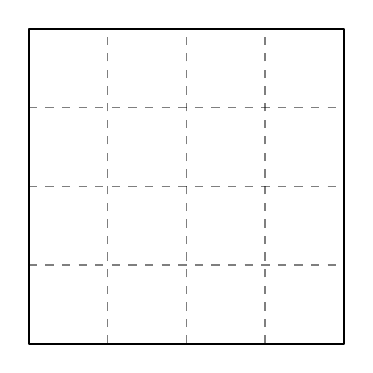
\begin{tikzpicture}[line join=bevel,scale=2,>=latex]
  \coordinate (n0) at (-1,-1);
  \coordinate (n1) at (1,-1);
  \coordinate (n2) at (1,1);
  \coordinate (n3) at (-1,1);

  \coordinate (n4) at (-0.5, -1);
  \coordinate (n5) at (0, -1);
  \coordinate (n6) at (0.5, -1);

  \coordinate (n7) at (1, -0.5);
  \coordinate (n8) at (1, 0);
  \coordinate (n9) at (1, 0.5);

  \coordinate (n10) at (0.5, 1);
  \coordinate (n11) at (0, 1);
  \coordinate (n12) at (-0.5, 1);

  \coordinate (n13) at (-1, 0.5);
  \coordinate (n14) at (-1, 0);
  \coordinate (n15) at (-1, -0.5);

  \coordinate (n16) at (-0.5, -0.5);
  \coordinate (n17) at (0, -0.5);
  \coordinate (n18) at (0.5, -0.5);

  \coordinate (n19) at (-0.5, 0);
  \coordinate (n20) at (0, 0);
  \coordinate (n21) at (0.5, 0);

  \coordinate (n22) at (-0.5, 0.5);
  \coordinate (n23) at (0, 0.5);
  \coordinate (n24) at (0.5, 0.5);
  
  
  \draw[thick] (n0) -- (n1) -- (n2) -- (n3) -- cycle;
  \draw[dashed,opacity=0.5] (n4) -- (n12);
  \draw[dashed,opacity=0.5] (n5) -- (n11);
  \draw[dashed,opacity=0.5] (n6) -- (n10);
  \draw[dashed,opacity=0.5] (n15) -- (n7);
  \draw[dashed,opacity=0.5] (n14) -- (n8);
  \draw[dashed,opacity=0.5] (n13) -- (n9);

  \nodeLabel{n0}{0}{black};
  \nodeLabel{n1}{1 }{black};
  \nodeLabel{n2}{2 }{black};
  \nodeLabel{n3}{3 }{black};
  \nodeLabel{n4}{4 }{red};
  \nodeLabel{n5}{5 }{red};
  \nodeLabel{n6}{6 }{red};
  \nodeLabel{n7}{7 }{red};
  \nodeLabel{n8}{8 }{red};
  \nodeLabel{n9}{9 }{red};
  \nodeLabel{n10}{10}{red};
  \nodeLabel{n11}{11}{red};
  \nodeLabel{n12}{12}{red};
  \nodeLabel{n13}{13}{red};
  \nodeLabel{n14}{14}{red};
  \nodeLabel{n15}{15}{red};
  
  \nodeLabel{n16}{16}{blue};
  \nodeLabel{n17}{17}{blue};
  \nodeLabel{n18}{18}{blue};
  \nodeLabel{n19}{19}{blue};
  \nodeLabel{n20}{20}{blue};
  \nodeLabel{n21}{21}{blue};
  \nodeLabel{n22}{22}{blue};
  \nodeLabel{n23}{23}{blue};
  \nodeLabel{n24}{24}{blue};

\end{tikzpicture}
        \caption{Node ordering given for a 4th order quad element with mid-edge and mid-face nodes.}
        \label{fig:ho_quad-numbered}
    \end{subfigure}
    \begin{subfigure}[b]{0.45\textwidth}
        \centering
        \newcommand{\nodeLabel}[3]{
    \node[color=#3, fill=white, opacity=0.9] at (#1) {\fontsize{10}{10}\selectfont #2}
}

\newcommand{\drawOffsetArrow}[2]{%
  \draw[->, color=red, thick] 
    ($ (#1)!0.1!(#2) $)  -- ($ (#2)!0.1!(#1) $)
}

\newcommand{\drawTri}[3]{
    \coordinate (midMid) at ($  ($(#1) !0.5! (#2)$)  !0.33!  (#3)  $);
    \coordinate (l0) at ($ (#1) !0.4! (midMid) $);
    \coordinate (l1) at ($ (#2) !0.4! (midMid) $);
    \coordinate (l2) at ($ (#3) !0.4! (midMid) $);
    \coordinate (l3) at ($ (l2) !0.33! (l0) $);
    \draw[->, color=blue, thick] (l0) -- (l1) -- (l2) -- (l3)
}

\newcommand{\drawTriFace}[4]{
    \coordinate (midMid) at ($  ($(#1) !0.5! (#2)$)  !0.33!  (#3)  $);
    \coordinate (l0) at ($ (#1) !0.4! (midMid) $);
    \coordinate (l1) at ($ (#2) !0.4! (midMid) $);
    \coordinate (l2) at ($ (#3) !0.4! (midMid) $);
    \coordinate (l3) at ($ (l2) !0.33! (l0) $);
    \nodeLabel{midMid}{#4}{blue};
    \draw[->, color=blue, thick] (l0) -- (l1) -- (l2) -- (l3)
}


\begin{tikzpicture}[line join=bevel,scale=2,>=latex]
  \coordinate (n0) at (-1,-1);
  \coordinate (n1) at (1,-1);
  \coordinate (n2) at (-1,1);
  
  \coordinate (l0) at (-0.75, -0.75);
  \coordinate (l1) at (0.3, -0.75);
  \coordinate (l2) at (-0.75, 0.3);
  \coordinate (l3) at (-0.75, -0.2);
  
%  \draw[thick] (n0) -- (n1) -- (n2) -- cycle;
  \drawOffsetArrow{n0}{n1};
  \drawOffsetArrow{n1}{n2};
  \drawOffsetArrow{n2}{n0};
  \drawTri{n0}{n1}{n2};

  \nodeLabel{n0}{0 }{black};
  \nodeLabel{n1}{1 }{black};
  \nodeLabel{n2}{2 }{black};

\end{tikzpicture}

        \caption{Orientation of tri face is indicated by the arrow (0 $\rightarrow$ 1 $\rightarrow$ 2 $\rightarrow$ 3).}
        \label{fig:ho_tri-arrow}
    \end{subfigure}
    \hfill
    \begin{subfigure}[b]{0.45\textwidth}
        \centering
        \newcommand{\nodeLabel}[3]{
    \node[color=#3, fill=white, opacity=0.9] at (#1) {\fontsize{10}{10}\selectfont #2}
}

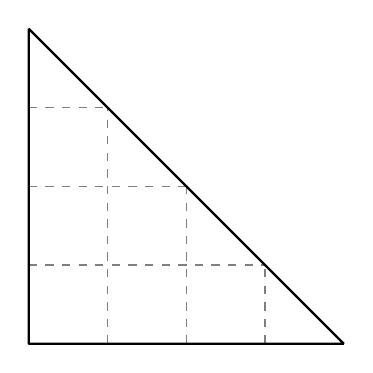
\begin{tikzpicture}[line join=bevel,scale=2,>=latex]
  \coordinate (n0) at (-1,-1);
  \coordinate (n1) at (1,-1);
  \coordinate (n2) at (-1,1);

  \coordinate (n3) at (-0.5, -1);
  \coordinate (n4) at (0, -1);
  \coordinate (n5) at (0.5, -1);

  \coordinate (n6) at (0.5, -0.5);
  \coordinate (n7) at (0, 0);
  \coordinate (n8) at (-0.5, 0.5);

  \coordinate (n9) at (-1, 0.5);
  \coordinate (n10) at (-1, 0);
  \coordinate (n11) at (-1, -0.5);

  \coordinate (n12) at (-0.5, -0.5);
  \coordinate (n13) at (0, -0.5);
  \coordinate (n14) at (-0.5, 0);  
  
  \draw[thick] (n0) -- (n1) -- (n2) -- cycle;
  \draw[dashed,opacity=0.5] (n3) -- (n8);
  \draw[dashed,opacity=0.5] (n4) -- (n7);
  \draw[dashed,opacity=0.5] (n5) -- (n6);
  \draw[dashed,opacity=0.5] (n11) -- (n6);
  \draw[dashed,opacity=0.5] (n10) -- (n7);
  \draw[dashed,opacity=0.5] (n9) -- (n8);

  \nodeLabel{n0}{0 }{black};
  \nodeLabel{n1}{1 }{black};
  \nodeLabel{n2}{2 }{black};
  \nodeLabel{n3}{3 }{red};
  \nodeLabel{n4}{4 }{red};
  \nodeLabel{n5}{5 }{red};
  \nodeLabel{n6}{6 }{red};
  \nodeLabel{n7}{7 }{red};
  \nodeLabel{n8}{8 }{red};
  \nodeLabel{n9}{9 }{red};
  \nodeLabel{n10}{10}{red};
  \nodeLabel{n11}{11}{red};
  \nodeLabel{n12}{12}{blue};
  \nodeLabel{n13}{13}{blue};
  \nodeLabel{n14}{14}{blue};


\end{tikzpicture}
        \caption{Node ordering given for a 4th order tri element with mid-edge and mid-face nodes.}
        \label{fig:ho_tri-numbered}
    \end{subfigure}
    \caption{Node ordering rules for higher order quad and tri elements}
    \label{fig:ho_2D_elements}
\end{figure}

Using the edge and face definitions in fig \ref{fig:ho_3D_elements},
we can derive the node ordering for higher order 3D elements too. As
in the 2D case, it is a concatenation of the vertices, then all the
mid-edge nodes, then all the mid-face nodes (if included) then all the
mid-volume nodes (if included).

\begin{figure}[h!]
    \centering
    \begin{subfigure}[b]{0.45\textwidth}
        \centering
        \newcommand{\nodeLabel}[3]{
    \node[color=#3, fill=white] at (#1) {\fontsize{10}{10}\selectfont #2}
}

\newcommand{\drawEdge}[3]{%
  \draw[->, color=red, thick] 
    ($ (#1)!0.1!(#2) $)  -- ($ (#2)!0.1!(#1) $);
  \nodeLabel{$(#1)!0.5!(#2)$}{#3}{red}
}

\newcommand{\drawTriFace}[5]{
    \coordinate (midMid) at ($  ($(#1) !0.5! (#2)$)  !0.33!  (#3)  $);
    \coordinate (l0) at ($ (#1) !#5! (midMid) $);
    \coordinate (l1) at ($ (#2) !#5! (midMid) $);
    \coordinate (l2) at ($ (#3) !#5! (midMid) $);
    \coordinate (l3) at ($ (l2) !0.33! (l0) $);
    \node[color=blue] at (midMid) {\fontsize{10}{10}\selectfont #4};
    \draw[->, color=blue, thick] (l0) -- (l1) -- (l2) -- (l3)
}

\tdplotsetmaincoords{63}{63}

\begin{tikzpicture}[line join=bevel,tdplot_main_coords,scale=2.2,>=latex]
  \coordinate (A) at (-1.5,-1.5,-1.5);
  \coordinate (B) at ( 1.5,-1.5,-1.5);
  \coordinate (C) at (0, 1.5,-1.5);
  \coordinate (D) at (0,-0.5, 1.5);

  \draw[dashed,opacity=0.5] (A) -- (C);
  \drawTriFace{A}{B}{C}{0}{0.3};
  \drawEdge{A}{C}{2};
  \drawTriFace{A}{B}{D}{1}{0.6};
  \draw (A) -- (B) -- (D) -- cycle;
  \drawTriFace{B}{C}{D}{2}{0.5};
  \drawTriFace{A}{C}{D}{3}{0.3};
  \draw (B) -- (C) -- (D);
  \drawEdge{A}{B}{0};
  \drawEdge{B}{C}{1};
  \drawEdge{A}{D}{3};
  \drawEdge{B}{D}{4};
  \drawEdge{C}{D}{5};
  \nodeLabel{A}{0}{black};
  \nodeLabel{B}{1}{black};
  \nodeLabel{C}{2}{black};
  \nodeLabel{D}{3}{black};

\end{tikzpicture}

        \caption{High-order tet}
        \label{fig:ho_tet}
    \end{subfigure}
    \hfill
    \begin{subfigure}[b]{0.45\textwidth}
        \centering
        \input{assets/HOprism.tex}
        \caption{High-order prism}
        \label{fig:ho_prism}
    \end{subfigure}
    \begin{subfigure}[b]{0.45\textwidth}
        \centering
       \resizebox{1.25\textwidth}{!}{\newcommand{\nodeLabel}[3]{
    \node[color=#3, fill=white] at (#1) {\fontsize{10}{10}\selectfont #2}
}

\newcommand{\drawEdge}[3]{%
  \draw[->, color=red, thick] 
    ($ (#1)!0.1!(#2) $)  -- ($ (#2)!0.1!(#1) $);
  \nodeLabel{$(#1)!0.5!(#2)$}{#3}{red}
}

\newcommand{\drawQuadFace}[6]{
    \coordinate (midMid) at ($  ($(#1) !0.5! (#2)$)  !0.5!  ($(#3) !0.5! (#4)$)  $);
    \coordinate (l0) at ($ (#1) !#6! (midMid) $);
    \coordinate (l1) at ($ (#2) !#6! (midMid) $);
    \coordinate (l2) at ($ (#3) !#6! (midMid) $);
    \coordinate (l3) at ($ (#4) !#6! (midMid) $);
    \coordinate (l4) at ($ (l3) !0.33! (l0) $);
    \node[color=blue] at (midMid) {\fontsize{10}{10}\selectfont #5};
    \draw[->, color=blue, thick] (l0) -- (l1) -- (l2) -- (l3)-- (l4)
}

\newcommand{\drawTriFace}[5]{
    \coordinate (midMid) at ($  ($(#1) !0.5! (#2)$)  !0.33!  (#3)  $);
    \coordinate (l0) at ($ (#1) !#5! (midMid) $);
    \coordinate (l1) at ($ (#2) !#5! (midMid) $);
    \coordinate (l2) at ($ (#3) !#5! (midMid) $);
    \coordinate (l3) at ($ (l2) !0.33! (l0) $);
    \node[color=blue] at (midMid) {\fontsize{10}{10}\selectfont #4};
    \draw[->, color=blue, thick] (l0) -- (l1) -- (l2) -- (l3)
}

\tdplotsetmaincoords{65}{50}

\begin{tikzpicture}[line join=bevel,tdplot_main_coords,scale=2.2,>=latex]
  \coordinate (A) at (-1.5,-1.5,-1.5);
  \coordinate (B) at ( 1.5,-1.5,-1.5);
  \coordinate (C) at ( 1.5, 1.5,-1.5);
  \coordinate (D) at (-1.5, 1.5,-1.5);
  \coordinate (E) at (   0,   0, 1.5);

  \draw[dashed,opacity=0.5] (A) -- (D) -- (C);
  \draw[dashed,opacity=0.5] (D) -- (E);
  \draw (A) -- (B) -- (C) -- (E) -- cycle;
  \draw (B) -- (E);

  \drawEdge{D}{C}{2};
  \drawEdge{A}{D}{3};
  \drawEdge{D}{E}{7};

  
  \drawQuadFace{A}{B}{C}{D}{0}{0.3};
  \drawTriFace{A}{B}{E}{1}{0.3};
  \drawTriFace{B}{C}{E}{2}{0.3};
  \drawTriFace{D}{C}{E}{3}{0.3};
  \drawTriFace{A}{D}{E}{4}{0.3};
  
  \drawEdge{A}{B}{0};
  \drawEdge{B}{C}{1};
  \drawEdge{A}{E}{4};
  \drawEdge{B}{E}{5};
  \drawEdge{C}{E}{6};

  \nodeLabel{A}{0}{black};
  \nodeLabel{B}{1}{black};
  \nodeLabel{C}{2}{black};
  \nodeLabel{D}{3}{black};
  \nodeLabel{E}{4}{black};

\end{tikzpicture}
}
        \caption{High-order pyra}
        \label{fig:ho_pyra}
    \end{subfigure}
    \hfill
    \begin{subfigure}[b]{0.45\textwidth}
        \centering
        \resizebox{1.1\textwidth}{!}{\newcommand{\nodeLabel}[3]{
    \node[color=#3, fill=white] at (#1) {\fontsize{10}{10}\selectfont #2}
}

\newcommand{\drawEdge}[3]{%
  \draw[->, color=red, thick] 
    ($ (#1)!0.1!(#2) $)  -- ($ (#2)!0.1!(#1) $);
  \nodeLabel{$(#1)!0.5!(#2)$}{#3}{red}
}

\newcommand{\drawQuadFace}[6]{
    \coordinate (midMid) at ($  ($(#1) !0.5! (#2)$)  !0.5!  ($(#3) !0.5! (#4)$)  $);
    \coordinate (l0) at ($ (#1) !#6! (midMid) $);
    \coordinate (l1) at ($ (#2) !#6! (midMid) $);
    \coordinate (l2) at ($ (#3) !#6! (midMid) $);
    \coordinate (l3) at ($ (#4) !#6! (midMid) $);
    \coordinate (l4) at ($ (l3) !0.33! (l0) $);
    \node[color=blue] at (midMid) {\fontsize{10}{10}\selectfont #5};
    \draw[->, color=blue, thick] (l0) -- (l1) -- (l2) -- (l3)-- (l4)
}

\tdplotsetmaincoords{65}{57}

\begin{tikzpicture}[line join=bevel,tdplot_main_coords,scale=2.2,>=latex]
  \coordinate (A) at (-1.2,-1.2,-1.2);
  \coordinate (B) at ( 1.2,-1.2,-1.2);
  \coordinate (C) at ( 1.2, 1.2,-1.2);
  \coordinate (D) at (-1.2, 1.2,-1.2);
  \coordinate (E) at (-1.2,-1.2, 1.2);
  \coordinate (F) at ( 1.2,-1.2, 1.2);
  \coordinate (G) at ( 1.2, 1.2, 1.2);
  \coordinate (H) at (-1.2, 1.2, 1.2);

  \draw[dashed,opacity=0.5] (A) -- (D) -- (C);
  \draw[dashed,opacity=0.5] (D) -- (H);
  \draw (A) -- (B) -- (F) -- (E) -- cycle;
  \draw (F) -- (G) -- (C) -- (B);
  \draw (E) -- (H) -- (G);

  \drawEdge{C}{D}{2};
  \drawEdge{D}{A}{3};
  \drawEdge{D}{H}{7};

  \drawQuadFace{A}{B}{C}{D}{0}{0.3};
  \drawQuadFace{A}{B}{F}{E}{1}{0.35};
  \drawQuadFace{B}{C}{G}{F}{2}{0.3};
  \drawQuadFace{D}{C}{G}{H}{3}{0.3};
  \drawQuadFace{A}{D}{H}{E}{4}{0.3};
  \drawQuadFace{E}{F}{G}{H}{5}{0.3};
  
  \drawEdge{A}{B}{0};
  \drawEdge{B}{C}{1};
  \drawEdge{A}{E}{4};
  \drawEdge{B}{F}{5};
  \drawEdge{C}{G}{6};
  \drawEdge{E}{F}{8};
  \drawEdge{F}{G}{9};
  \drawEdge{G}{H}{10};
  \drawEdge{H}{E}{11};

  \nodeLabel{A}{0}{black};
  \nodeLabel{B}{1}{black};
  \nodeLabel{C}{2}{black};
  \nodeLabel{D}{3}{black};
  \nodeLabel{E}{4}{black};
  \nodeLabel{F}{5}{black};
  \nodeLabel{G}{6}{black};
  \nodeLabel{H}{7}{black};

\end{tikzpicture}
}
        \caption{High-order hex}
        \label{fig:ho_hex}
    \end{subfigure}
    \caption{Node ordering rules for higher order 3D elements elements}
    \label{fig:ho_3D_elements}
\end{figure}

Mid-volume nodes are ordered in a similar fashion to mid-face
nodes. They are given slice-by-slice, parallel to and moving away from
face 0, and with the orientation dictated by face 0. This is most
easily seen in the example given in fig. \ref{fig:vol_nodes}. For pyra
and prisms, the slices are still quads, but with the size of/number of
nodes in each slice decreasing away from face 0. For tets, the slices
are triangular and with decreasing size.

\begin{figure}[h!]
  \centering
  \newcommand{\nodeLabel}[3]{
    \node[color=#3, fill=white] at (#1) {\fontsize{10}{10}\selectfont #2}
}

\newcommand{\noFillLabel}[3]{
    \node[color=#3] at (#1) {\fontsize{10}{10}\selectfont #2}
}

\newcommand{\drawQuadFace}[6]{
    \coordinate (midMid) at ($  ($(#1) !0.5! (#2)$)  !0.5!  ($(#3) !0.5! (#4)$)  $);
    \coordinate (l0) at ($ (#1) !#6! (midMid) $);
    \coordinate (l1) at ($ (#2) !#6! (midMid) $);
    \coordinate (l2) at ($ (#3) !#6! (midMid) $);
    \coordinate (l3) at ($ (#4) !#6! (midMid) $);
    \coordinate (l4) at ($ (l3) !0.33! (l0) $);
    \node[color=blue] at (midMid) {\fontsize{10}{10}\selectfont #5};
    \draw[->, color=blue, thick] (l0) -- (l1) -- (l2) -- (l3)-- (l4)
}

\newcommand{\volNode}[4]{
  \pgfmathsetmacro \dx{#1 / 4}
  \pgfmathsetmacro \dy{#2 / 4}
  \pgfmathsetmacro \dz{#3 / 4}
  \coordinate (tmp) at ($($($(A) !\dx! (B)$) !\dy! ($(D) !\dx! (C)$)$) 
                   !\dz! ($($(E) !\dx! (F)$) !\dy! ($(H) !\dx! (G)$)$)$);
  \noFillLabel{tmp}{#4}{green!80!black}
}

\tdplotsetmaincoords{68}{59}

\begin{tikzpicture}[line join=bevel,tdplot_main_coords,scale=2.2,>=latex]
  \coordinate (A) at (-1.2,-1.2,-1.2);
  \coordinate (B) at ( 1.2,-1.2,-1.2);
  \coordinate (C) at ( 1.2, 1.2,-1.2);
  \coordinate (D) at (-1.2, 1.2,-1.2);
  \coordinate (E) at (-1.2,-1.2, 1.2);
  \coordinate (F) at ( 1.2,-1.2, 1.2);
  \coordinate (G) at ( 1.2, 1.2, 1.2);
  \coordinate (H) at (-1.2, 1.2, 1.2);

  \draw[dashed,opacity=0.5] (A) -- (D) -- (C);
  \draw[dashed,opacity=0.5] (D) -- (H);
  
  \drawQuadFace{A}{B}{C}{D}{0}{0.3};
  
  \nodeLabel{D}{3}{black};
  
  \volNode{1}{1}{0.5}{98};
  \volNode{2}{1}{0.5}{99};
  \volNode{3}{1}{0.5}{100};
  \volNode{1}{2}{0.5}{101};
  \volNode{2}{2}{0.5}{102};
  \volNode{3}{2}{0.5}{103};
  \volNode{1}{3}{0.5}{104};
  \volNode{2}{3}{0.5}{105};
  \volNode{3}{3}{0.5}{106};
  \volNode{1}{1}{2}  {107};
  \volNode{2}{1}{2}  {108};
  \volNode{3}{1}{2}  {109};
  \volNode{1}{2}{2}  {110};
  \volNode{2}{2}{2}  {111};
  \volNode{3}{2}{2}  {112};
  \volNode{1}{3}{2}  {113};
  \volNode{2}{3}{2}  {114};
  \volNode{3}{3}{2}  {115};
  \volNode{1}{1}{3.5}{116};
  \volNode{2}{1}{3.5}{117};
  \volNode{3}{1}{3.5}{118};
  \volNode{1}{2}{3.5}{119};
  \volNode{2}{2}{3.5}{120};
  \volNode{3}{2}{3.5}{121};
  \volNode{1}{3}{3.5}{122};
  \volNode{2}{3}{3.5}{123};
  \volNode{3}{3}{3.5}{124};

  \draw (A) -- (B) -- (F) -- (E) -- cycle;
  \draw (F) -- (G) -- (C) -- (B);
  \draw (E) -- (H) -- (G);
  
  \nodeLabel{A}{0}{black};
  \nodeLabel{B}{1}{black};
  \nodeLabel{C}{2}{black};
  \nodeLabel{E}{4}{black};
  \nodeLabel{F}{5}{black};
  \nodeLabel{G}{6}{black};
  \nodeLabel{H}{7}{black};

\end{tikzpicture}

  \caption{Volume node ordering for a 4th order hex element}
  \label{fig:vol_nodes}
\end{figure}

\section{Input Modules}
As well as being able to generate meshes in NekMesh, we seek to make
NekMesh compatible with multiple commonly-used file formats, enabling
users to create meshes in their chosen mesh generation software,
before either elevating their order in NekMesh or using it as is. Some
file formats provide an API for reading from (and writing to) them;
this includes .ccm with CCMIO and .cgns with CGNS Mid-Level
Library. Other formats such as .gmsh do not, so we must manually read
the file with \texttt{stringstream}. Once the required information
(such as node coordinates, elements nodes, boundary conditions etc.)
has been read from the file, however, the process is the same:

\begin{enumerate}
\item For each node we must first create a node shared pointer
  (\texttt{NodeSharedPtr}) append it to \texttt{m\_node} and insert it
  into \texttt{vertexSet} eg.\\
\begin{lstlisting}[style=BashInputStyle]
NodeSharedPtr newNode = std::make_shared<Node>(id, x, y, z);
m_mesh->m_node.push_back(newNode);
m_mesh->m_vertexSet.insert(newNode);
\end{lstlisting}
 
...\textbf{ensuring} that the node IDs all comply with the Prism and
Pyramid rules (section \ref{sect:node_ordering}).

\item We must then append an ElementSharedPtr for each element
  (internal \textit{and} boundary), eg.
\begin{lstlisting}[style=BashInputStyle]
ElementSharedPtr E = GetElementFactory().CreateInstance(elType, conf,
nodeList, tags); m_mesh->m_element[E->GetDim()].push_back(E);
\end{lstlisting}

\item Once the elements and nodes have been correctly created, the
  following functions are called sequentially to process this
  information into the NekMesh format.
\begin{lstlisting}[style=BashInputStyle]
ProcessEdges();
ProcessFaces(); 
ProcessElements(); 
ProcessComposites(); 
\end{lstlisting}
\end{enumerate}

\subsection{StarCCM+ .ccm input (InputStar.cpp)}

\subsection{Gmsh .msh input (InputGmsh.cpp)}

\subsection{CGNS .cgns input (InputCGNS.cpp)}
Information about the CGNS Standard Interface Data Structure (SIDS)
can be found at
\url{https://cgns.github.io/CGNS_docs_current/sids}. This converter
makes use of the CGNS Mid-Level Library and information about that can
be found at \url{https://cgns.github.io/CGNS_docs_current/midlevel}.We
will summarise the key points about the CGNS standard.\\

Every file will contain at least one zone, which contains information
about coordinates and the mesh. Each zone contains at least one base,
which contain information about the information about the
dimensionality of the domain (fig. \ref{fig:cgn-db-hierarchy}).

\begin{figure}[h]
 \centering
  \includegraphics[width=0.6\textwidth]{img/CGNS_database_hierarchy.png}
  \caption{CGNS database hierarchy. Image from cgns.github.io}
  \label{fig:cgns-db-hierarchy}
\end{figure}

Elements are stored in sections where they are grouped by element type
in the case of SEPARATED CGNS files or all the elements are grouped
together in the case of a MIXED CGNS file. Depending on the file
format, the \texttt{InputCGNS.cpp} either uses ExtractMixedElemInfo()
or ExtractSeparatedElemInfo(). In both case, an array
\texttt{ElementConnectivity} is read in, containing the node IDs for
each element (in the MIXED format the element type must also be
specified for each element). Each function takes the
\texttt{ElementConnectivity} array and generates a vector
\texttt{elemInfo} which contains the type and node list for each
element.\\

The function ReadFaces converts from \texttt{elemInfo} into a face
representation, where each element is defined by its face
(\texttt{ElementFaces}), each face is defined by its nodes
(\texttt{FaceNodes}), and the boundary element faces of the mesh are
stored in \texttt{BndElementFaces}. These three variables are required
for the next function \texttt{ResetNodes} and allows us to re-use a
large section of code from the \texttt{InputStar} converter. \\

The final step that must be mentioned is the fact that CGNS and
NekMesh use different conventions for the order in which to list
higher order nodes. In the functions \texttt{GenElement2D} and
\texttt{GenElement3D}, we must use mappings generated by
\texttt{CGNSReordering} to map between the diffent
conventions. Although these could be produced algorithmically (and one
would want to if CGNS supported orders higher than 4th), for the
moment they have been hard-coded in by manually comparing the node
orderings in the CGNS SIDS \cite{SIDS_node_ordering} and NekMesh
\ref{sect:HO_node_ordering}.

%\subsection{CCM/CGNS shared base class (InputStarCGNS.cpp)}
%\texttt{ResetNodes} is the function responsible with renumbering the
%node IDs in accordance with the rules in section \ref{}. It requires
%the variables \texttt{ElementFaces} and \texttt{FaceNodes}, which are
%created differently in the two input modules, since .ccm and .cgns
%store elements differently.\\ \texttt{CreateElements} creates the 3D
%and then 2D elements

\section{Process Modules}
\section{Output Modules}


\begin{thebibliography}{References}
 \bibitem{NekMesh_paper} NekMesh: An open-source high-order mesh generation framework
 \bibitem{textbook} George Karniadakis, Spencer Sherwin, \textit{Spectral/hp Element Methods for Computational Fluid Dynamics}
 \bibitem{SIDS_node_ordering}\url{ https://cgns.github.io/CGNS_docs_current/sids/conv.html\#unstructgrid}
\end{thebibliography}

%\end{document}
